\subsection{重味夸克半轻子衰变}

在强子衰变模拟当中,除了来源于强子衰变的双电子以外,另一个很重要的部分就是来源于重味夸克半轻子衰变的双电子。重味夸克半轻子衰变在双电子谱的分析中主要包括璨夸克和底夸克的半轻子衰变过程。在较低的对撞质心能量下,底夸克的反应截面远小于璨夸克的反应截面,可以忽略不计,在本分析当中仅对璨夸克的半轻子衰变过程进行模拟。在模拟时首先用Pythia模拟得到璨夸克的半轻子衰变在$\sqrt{s_{\mathrm{NN}}} = 54.4 \rm{GeV}$质子-质子对撞中的双电子谱,再经过反应截面和二元对撞数($N_{bin}$)的归一化之后得到金-金对撞情况下的双电子谱。具体模拟方法将在下文进行讨论。

首先是Pythia产生子的设置,本分析当中所用的Pythia基本沿用了STAR实验当中模拟所使用的默认参数,并对下列的参数进行了调整以使其可以更好的描述测量结果\cite{PhysRevD.86.072013}。被调整的参数以及具体的值如下所示
\begin{itemize}
    \item MSEL = 4(c trigger) 
    \item PARP(91) = 1 $<k_T>$ = 1.0 GeV/c
    \item PARP(61) = 1 (Parton shower level tuning)
\end{itemize}
同时为了提高模拟的效率,将模拟过程中含璨夸克的介子不包含电子的衰变道关闭。

当模拟得到来源于璨夸克半轻子衰变的双电子谱之后,需要对其进行归一化之后才能得到可以和测量结果进行比较的双电子谱。Pythia模拟得到的是在
归一化方程如式\ref{eq:Nor_c}所示。其中$\sigma_{c\bar{c}}$和$\sigma_{mb}$分别为金-金对撞中璨夸克和最小无偏对撞的截面。$N_{bin}$为不同中心度下的二元碰撞数,添加此归一化因子的原因是将金-金对撞等效为$N_{bin}$次质子-质子对撞。$N_{bin}$具体数值由STAR官方的中心度定义包给出,在不同中心度下的结果如表\ref{tab:Nbin}所示。BR为含璨夸克的介子包含电子或者正电子衰变道的分支比。

\begin{equation}
    \label{eq:Nor_c}
    \frac{dN}{dM} = \frac{1}{N_{evt}} \frac{\sigma_{c\bar{c}}}{\sigma_{mb}} (\frac{dN}{dM})_{pp} N_{bin} (BR_{c~\rightarrow e^+}) (BR_{c~\rightarrow e^-})
\end{equation}

在本小节接下来的部分会对归一化方程中的一些归一化因子进行具体的讨论。

首先是 $\frac{1}{N_{evt}}$, 即总事例数归一化因子。在确定$N_{evt}$的时候两种不同的方法,分别为
\begin{itemize}
    \item 璨夸克事例方法(inclusive charm method), $N_{evt}$为模拟时至少有一个璨夸克或者反璨夸克的事例数
    \item 两璨弦事例方法(2 c string method), $N_{evt}$为模拟时同时具有有一个c string 和 $\bar{c}$ string的事例数
\end{itemize}

当强子衰变模拟的结果和测量结果进行比较的时候,其纵轴为$dN/dM_{ee}$。其物理意义为一次最小无偏对撞中的双电子的产额。所以在做模拟的归一化时,所用的总事例数$N_{evt}$应该满足式\ref{eq:N_decay}。这就要求在选择$N_{evt}$时应该和计算$\sigma_{c\bar{c}}$时的总事例数选择方法相同。测量$\sigma_{c\bar{c}}$\cite{STAR:2012nbd}的方法首先是通过测量open charm的产额,再通过其确定璨夸克在中间快度区域(mid rapidity)的截面。最后通过这个中间快度区域的截面反推得到全空间的截面。基于此测量方法,$N_{evt}$应该为模拟当中可以发现open charm的事例数。在检查Pythia模拟的整个工作流之后可以发现,当没有两个c string产生的时候,仍然可以在末态找到来源于open charm的电子对。也就是说璨夸克事例方法是一个更加合理的确定$N_{evt}$的方法。
\begin{equation}
    \label{eq:N_decay}
    N_{mb} = N_{evt}*\frac{\sigma_{mb}}{\sigma_{c\bar{c}}}
\end{equation}

正如在绪论当中讨论到的,质子-质子中的双电子谱测量可以为重离子对撞中的双电子谱测量定下一条很好的基线。\ref{fig:STARpp}为\sNN = 200 GeV质子-质子对撞中的双电子谱测量结果\cite{Guo:2014rba}。可以看到在此分析当中来自于重味夸克的模拟结果可以很好的在中等质量区间内描述数据。在此分析当中所使用的确定$N_{evt}$的方法正是璨夸克事例方法。在对其模拟结果进行重复的时候也可以发现当用璨夸克事例方法来确定$N_{evt}$时,模拟结果可以更好的描述质子-质子对撞中的双电子谱,如图\ref{fig:Charm_reproduce}所示。

\begin{figure}[htb]
    \begin{center}
    \includegraphics[width=0.8\textwidth,clip]{figures/Chapter4/Charm_reproduce.png}
    \end{center}
    \caption[\sNN = 200 GeV质子-质子双电子谱测量结果与璨夸克不同模拟方法比较示意图]{\sNN = 200 GeV质子-质子对庄重璨夸克不同模拟方法比较示意图。其中黑色和蓝色实心点分别为STAR Run9双电子谱测量中的数据点和模拟结果\cite{STAR:2012dzw}。红色实心点为\ref{fig:STARpp}中的模拟结果。红色空心点和玫红色三角分别为用两重不同的选择方法对\sNN = 200 GeV当中的璨夸克产额进行模拟的结果}
    \label{fig:Charm_reproduce}
\end{figure}

其次是$\sigma_{c\bar{c}}$ 。$\sigma_{c\bar{c}}$在此分析中面临和前文中提到的强子横动量谱以及强子产额一样的问题,缺少在此能量下的数据测量。所以在本分析当中使用的$\sigma_{c\bar{c}}$也是通过外推的手段得到。其他合作组和STAR实验已经有了在许多对撞能量下的$\sigma_{c\bar{c}}$测量结果,对于\sNN = 54.4 GeV金-金对撞当中的$\sigma_{c\bar{c}}$可以通过拟合这些数据的方式外推得到。拟合结果如图\ref{fig:Charm_Xsection}所示。通过拟合得到54.4 GeV金-金对撞当中的$\sigma_{c\bar{c}}$值为${\rm 72.49~\mu b}$。
\begin{figure}[htb]
    \begin{center}
    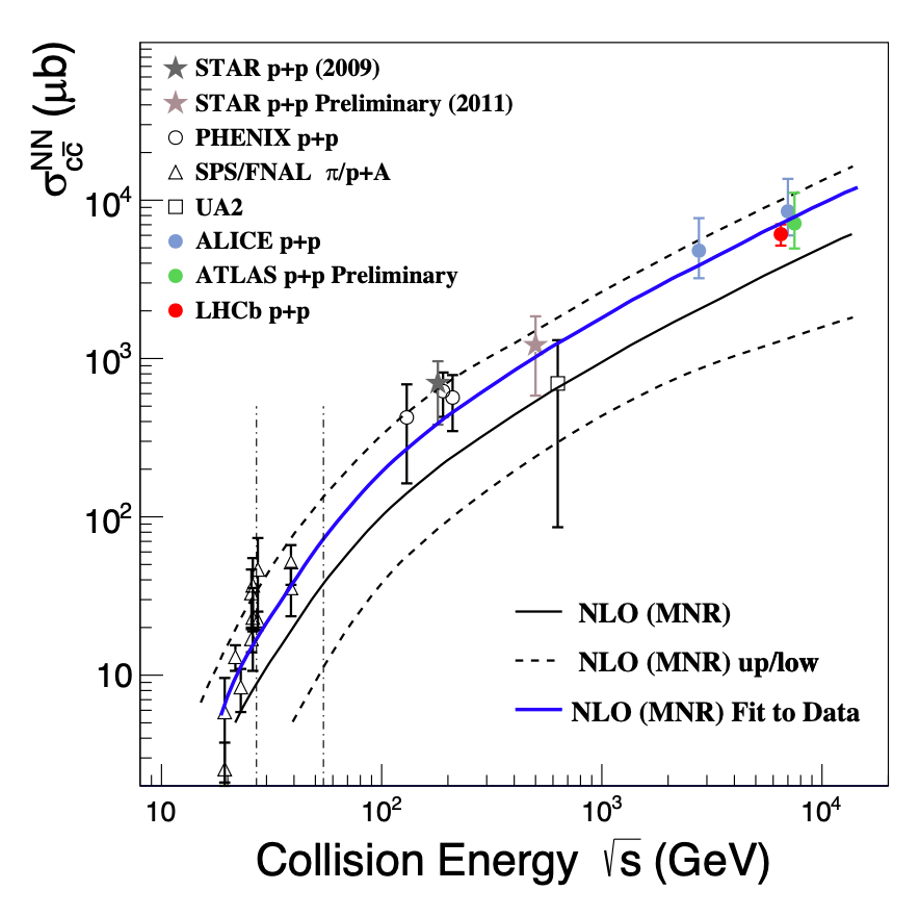
\includegraphics[width=0.8\textwidth,clip]{figures/Chapter4/CharmXsession.png}
    \end{center}
    \caption[$\sigma_{c\bar{c}}$拟合结果]{$\sigma_{c\bar{c}}$拟合结果,拟合曲线为NLO(MNR)理论计算曲线}
    \label{fig:Charm_Xsection}
\end{figure}
\begin{table}[h!]
    \centering
    \caption{\sNN = 54.4 GeV 金-金对撞中不同中心度下$N_{bin}$的值}
    \label{tab:Nbin}
    \begin{tabularx}{0.8\textwidth} {
    | >{\centering\arraybackslash}X  |>{\centering\arraybackslash}X | }
    \hline
    Centrality & $N_{bin}$ \\
    \hline
    0-80\% & 257.20 \\
    \hline
    0-10\% & 811.80 \\
    \hline
    10-40\% & 342.06 \\
    \hline
    40-80\% & 51.22 \\
    \hline
    \end{tabularx}
\end{table}

最后, $\sigma_{mb}$ 依然缺少在\sNN = 54.4 GeV下的数据测量结果。同样是采用拟合在其他能量下的$\sigma_{mb}$方式来外推\sNN = 54.4 GeV下的$\sigma_{mb}$结果。拟合结果如图\ref{fig:mbXSecFit}所示,拟合得到的\sNN = 54.4 GeV下$\sigma_{mb}$为35.17 mb。
\begin{figure}[htb!]
    \begin{center}
    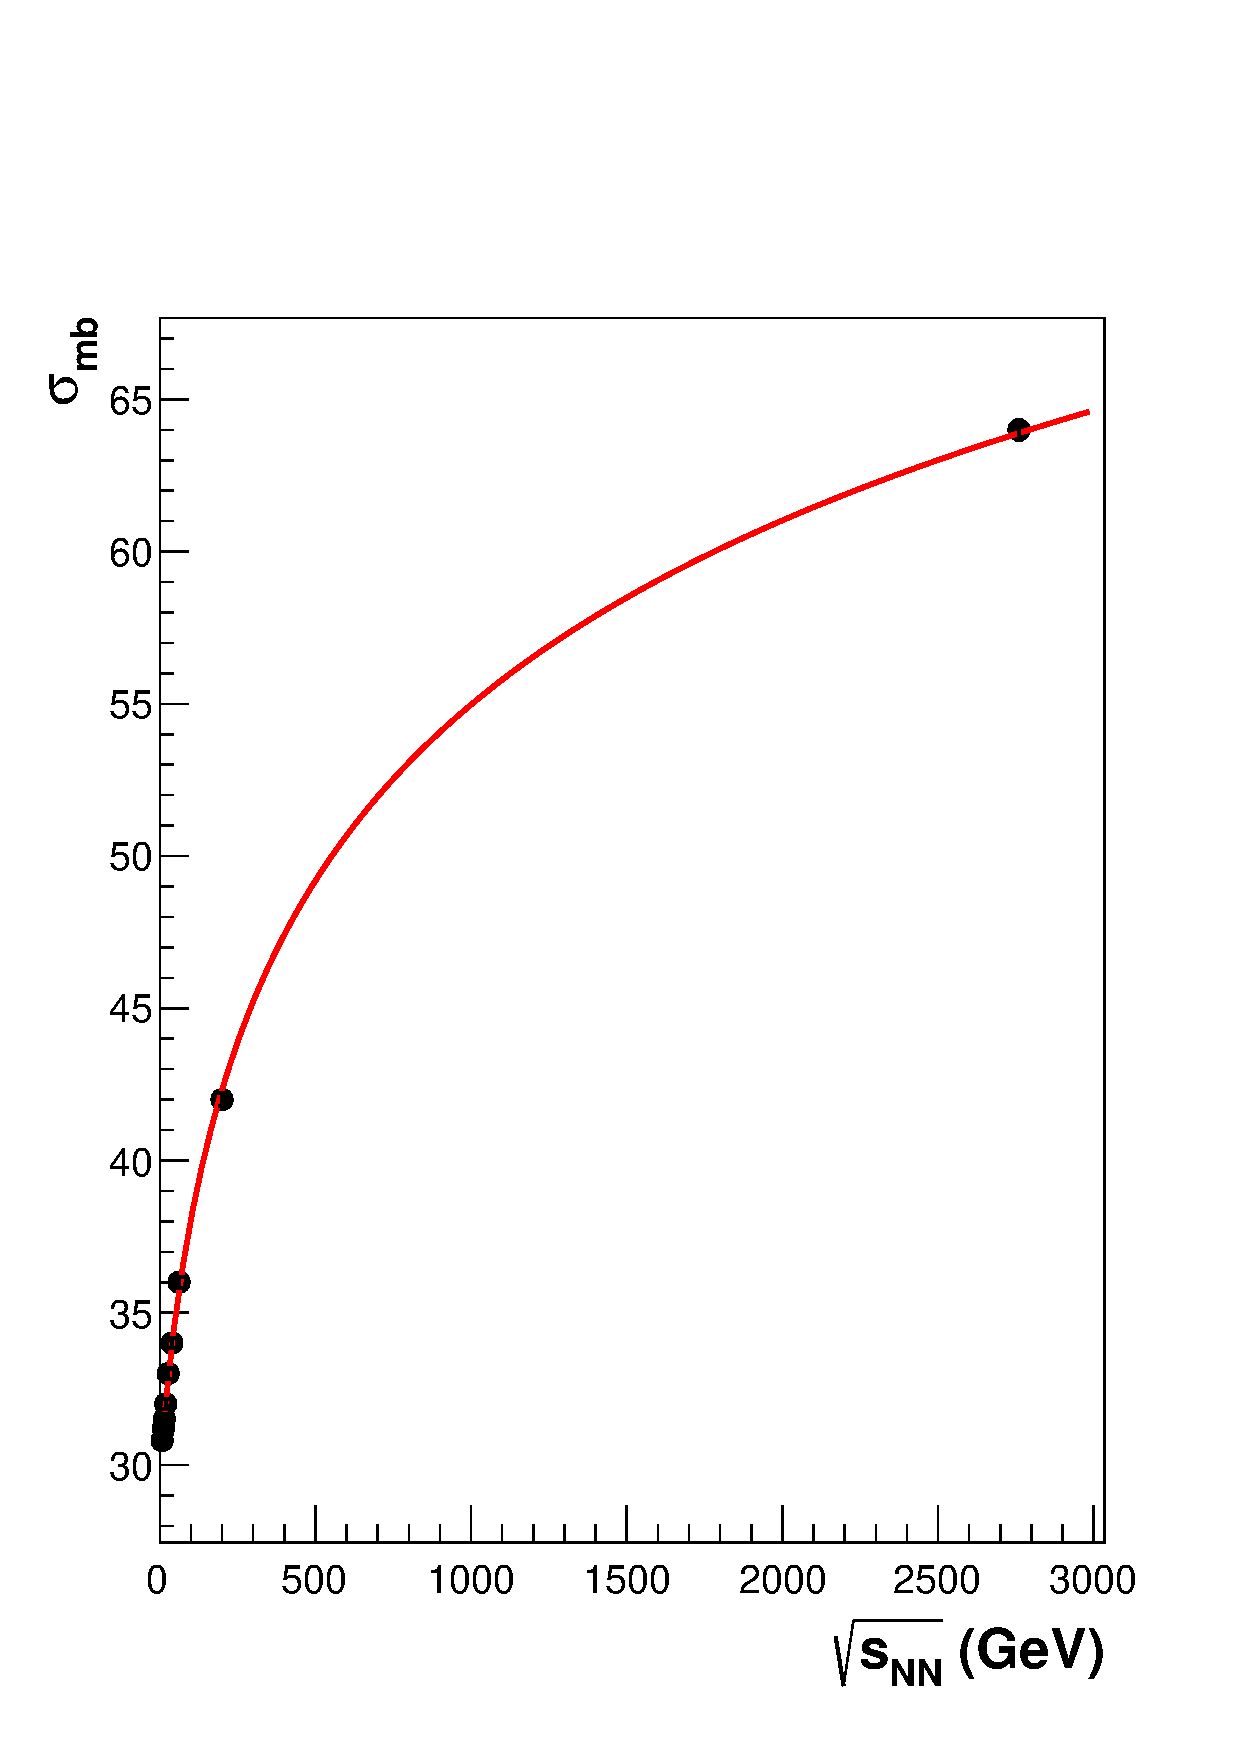
\includegraphics[width=0.7\textwidth,clip]{figures/Chapter4/mbXSecFit.pdf}
    \end{center}
    \caption[$\sigma_{mb}$拟合结果]{$\sigma_{mb}$拟合结果}
    \label{fig:mbXSecFit}
\end{figure}


